%Jazz IMU Report Template
%M. McDonald 3/2/17

\documentclass[14pt,a4paper]{article}
\usepackage{graphicx}
\usepackage[usenames, dvipsnames]{color}
\usepackage{float}
\usepackage{amsmath}
%fonts:
\newcommand*{\CenturySchool}{\fontfamily{pnc}\selectfont}
\newcommand*{\Times}{\fontfamily{ptm}\selectfont}

%Cover Page Values:

%Document Number: (Project ID)-(System ID)-(System Document ID)
\newcommand{\docno}{JS-00-01}

%Document Name:
\newcommand{\docname}{General Requirements Documentation}

%User Name
\newcommand{\name}{Mitchel McDonald}

\begin{document}
	
	\begin{CenturySchool}
		%Jazz IMU Cover Page
%M. McDonald 3/2/17
%\usepackage{cmfib}
\definecolor{SlateBlue}{RGB}{45, 83, 154}	

\begin{titlepage}
	
	\centering
	\begin{CenturySchool}
		{\fontsize{48}{56}\selectfont\bfseries\textcolor{SlateBlue}{Jazz IMU}\par}
	\end{CenturySchool}
	
	\begin{Times}
		{\fontsize{28}{33}\selectfont{For High Power Rocketry}\par}
		\vspace{6cm}
		{\fontsize{28}{33}\selectfont\docno\par}
		{\fontsize{28}{33}\selectfont\docname\par}
		{\fontsize{28}{33}\selectfont\name\par}
	\end{Times}

\end{titlepage}
		
		\tableofcontents
		
		\section{Foreward}
		%\chapter{Foreward}
		The purpose of this document to establish the basic requirements of Jazz, an Inertial Measurement Unit (IMU) purpose-built for High Power Rocketry and similar applications. This will be described through the following:

		\begin{enumerate}
			\item Concept of Operations (Con-Ops)
			\item Establishment of a Work Breakdown Structure (WBS)
			\item List of basic requirements
			\item Requirement verification methodologies
		\end{enumerate}
		
		\section{Concept of Operations}
		To provide a greater contextualization of needed requirements, a relevant illustration is needed. This illustration comes in the form of a “Concept of Operations”, which describes the environment the Jazz IMU will be nominally operated, what actions that would need to be taken at the beginning of its lifetime to ensure this, as well as consider how the Jazz IMU will be used by the consumer base. It is presently assumed that the IMU will not contain any hazardous materials and thus it can be easily be disposed of. Thus, any end-of-life activities are considered out of scope of this document.
		
		\subsection{Nominal Operations}
		Nominal usage of the Jazz IMU would be within a high-power rocket on a suborbital parabolic flight path. Such vehicles are primarily the domain of the scientific community and rocket enthusiasts (i.e. Tripoli, NAR clubs).
		

		\begin{figure}[H]
			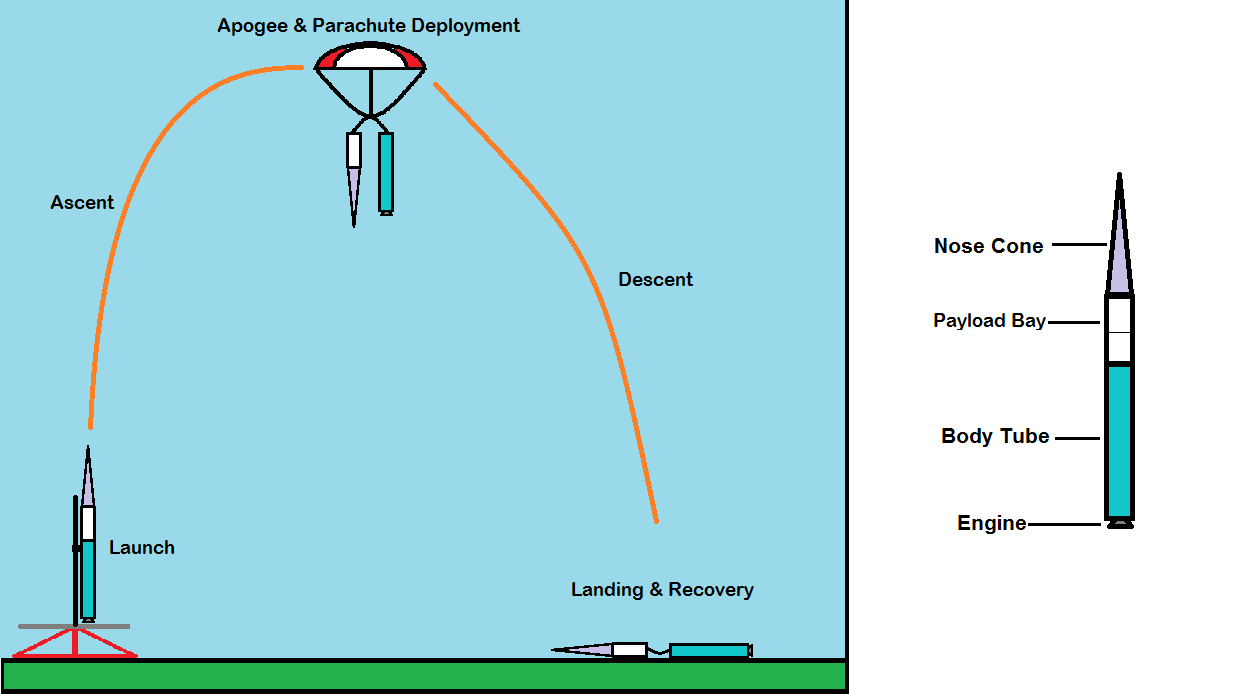
\includegraphics[width=\linewidth]{associated_files/Con_Ops_Opertions_Combo.png}
			\bfseries\caption{An outline of the phases of flight (L) and a description of a standard HPR vehicle (R)}
			\label{fig:img1)}
		\end{figure}

		
		In Figure 1 (R), a breakdown of the main components of a high power rocket are seen: 
		
		\begin{itemize}
		
		\item{\bfseries The Nose Cone:}  Present to enhance the aerodynamics of the vehicle.
		
		\item{\bfseries The Payload Bay:} Where the Jazz IMU will be stored. Like with all IMUs, Jazz will need to be firmly attached to its payload bay. Jazz will also need to be connected to a data collection device.
		
		\item{\bfseries The Body Tube:} The tube which contains the majority of the rocket’s dynamic components, including the engine, engine mount, ejection charge, and parachute.
		
		Henceforth, the terms rocket and vehicle will be used interchangeably.
		
		During nominal operations, the vehicle will undergo (5) phases of flight, as illustrated in Fig 1 (L): Launch, Ascent, Apogee \& Parachute Deployment, Descent, and Landing \& Recovery.
		
		\item{\bfseries Launch:} The inertial measurement unit will be initialized before launch, and may run for an indeterminate period of time while on the launch pad. 
		
		\item{\bfseries Ascent:} During ascent, the vehicle will experience a brief period of high acceleration and vibration from the engine, as well as perturbing forces from the surrounding atmosphere, which will be “seen” by the IMU. After the engine cutoff, the vehicle will continue to coast upward as it slowly decelerates toward apogee.
		
		\item{\bfseries Apogee \& Parachute Deployment:} Near apogee, a timed charge in the vehicle will separate the body tube from the payload/nosecone unit as well as eject a parachute. During this time, it is assumed that the vehicle will experience an acceleration “shock” from ejection.
		
		\item{\bfseries Descent:} After A\&PD, the vehicle will descend slowly to the landing point.
		
		\item{\bfseries Landing \& Recovery:} At landing, the vehicle will experience a final acceleration “shock” as it hits the ground. After that point, it will be assumed that the vehicle will remain motionless. Recovery of the vehicle and IMU will occur after an indeterminate period of time.
		
		\end{itemize}
		
		\subsection{Beginning of Life Activities} 
		To ensure that the end user receives an IMU that meets established specifications, each Jazz IMU will need to undergo calibration and functional testing.
		
		\subsection{Failure Modes}
		There is the distinct possibility that one that one or more parts of the Jazz IMU may fail during nominal operation. These failures can vary with, but are not limited to:
		
		\begin{enumerate}
			\item{Sensor failing to communicate with IMU microcontroller}
			
			\item{Sensor feeding IMU microcontroller bad data}
			
			\item{IMU microcontroller firmware crashing}
			
			\item{IMU performing incorrect processes}
			
			\item{Incorrect data output to acquisition devices}
		\end{enumerate}
		
		\subsection{Customer End Uses}
		As previously stated in 1.1, it is presently assumed that the primary customers using the Jazz IMU will be those in the scientific community launching a sounding rocket, or rocket club enthusiasts. Keeping these groups in mind, here are a few ideas as to what a customer would desire to use the Jazz IMU for.
		
		\begin{enumerate}
			\item {Vehicle Location Determination}
			\subitem{a. [Enthusiast/Scientist]: Linking the product to a radio platform to determine the landing site of the vehicle.}
			\subitem{b. [Enthusiast/Scientist]: Using position data to reconstruct a 3D flight path of the vehicle.}
			\subitem{c. [Enthusiast]: Using data to determine a high-fidelity apogee measurement.}
			
			\item{Attitude Determination}
			\subitem{a. [Scientist]: For vehicle trajectory determination}
			
			\item{Association of IMU data with other systems}
			\subitem{a.	[Scientist]: Cross referencing IMU data with other scientific platforms (i.e. environment measurement systems) on the vehicle.}
			
			\item{Vehicle Control}
			\subitem{a.	[Scientist]: Passing IMU data to a vehicle control system.}
		\end{enumerate}
				
		\section{Work Breakdown Structure}
			\begin{figure}[H]
				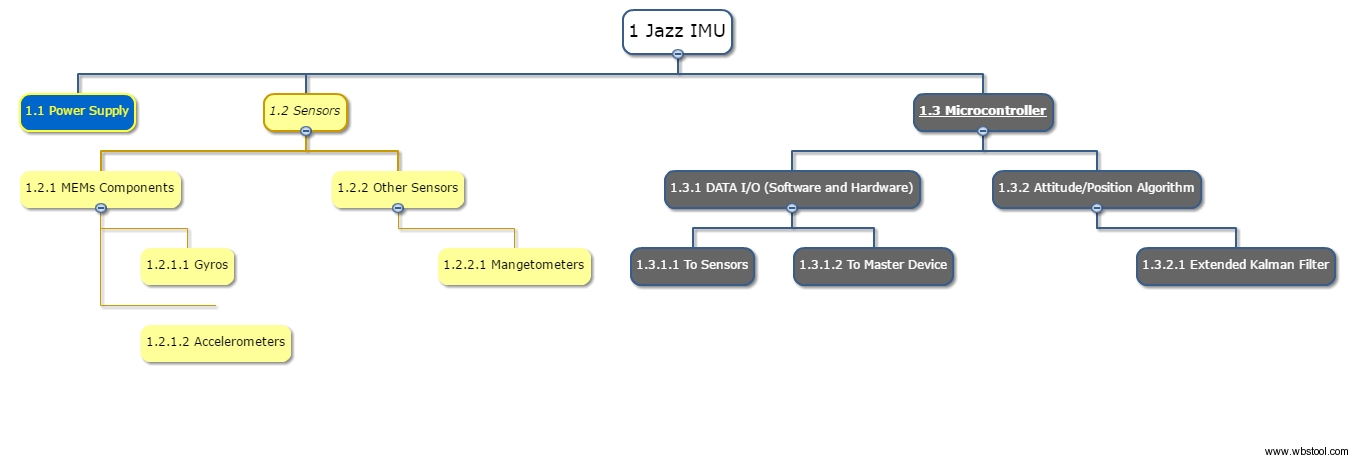
\includegraphics[width=\linewidth]{associated_files/Jazz_WBS.jpg}
				\bfseries\caption{}
				\label{fig:img1)}
			\end{figure}
		
		\section{Basic Requirements}
		
			\begin{enumerate}
				\item Jazz IMU shall use microelectromechanical (MEMs) accelerometers, gyroscopes, and magnetometers as its primary means of attitude and position determination.
				
				\item Jazz IMU shall be able to determine attitude within X degrees and within Y meters.
				
				\item Jazz IMU shall be resistant to extreme accelerations seen in a high power rocket flight, including continuous accelerations up to X Gs and “Jolts” up to Y Gs.
				
				\item Jazz IMU shall be resistant to extreme rates seen in a high power rocket flight, including continuous rates up to X m/s and “Jolts” up to Y m/s.
				
				\item Jazz IMU shall be able to run for X period of time without incurring an IMU software crash (Failure Mode 1.3.4).
				
				\item Jazz IMU shall be able to inform the user of hardware failure (Failure Mode 1.3.1).
				
				\item Jazz IMU shall be resistant to all other failure modes.
				
				\item Jazz IMU shall weigh only X Kg and take up a volume of no more than Y \(m^3\).
				 
			\end{enumerate}
			
			\section{Verfication Requirement Methodologies}
			
			The following instructions listed are methods to further define, verify, and validate the requirements in section 3. Note that these take place throughout the entire development process:
			
				\begin{enumerate}
					\item{\bfseries Jazz IMU shall use microelectromechanical (MEMs) accelerometers, gyroscopes, and magnetometers as its primary means of attitude and position determination.}
					\subitem a.	Only MEMs components will be considered in the selection process.
					\subitem b.	Simulations will need to accurately represent MEMs accelerometer/gyro properties.
					
					\item{\bfseries Jazz IMU shall be able to determine attitude within X degrees and within Y meters.}
					\subitem a.	Numerical establishment of this requirement is needed. This requirement can vary greatly, as one could follow precedent of ballistic missile INS design for a high-accuracy system, or an accuracy sufficient enough to meet the customer usages stated in 1.4. This requirement value may change greatly depending on what can be capably expected of the sensor.
					\subitem b.	V\&V using an environmental simulation.
					\subitem c.	V\&V using a test vehicle.
					
					
					\item{\bfseries Jazz IMU shall be resistant to extreme accelerations seen in a high power rocket flight, including continuous accelerations up to X Gs and “Jolts” up to Y Gs.}
					
					\item{\bfseries Jazz IMU shall be resistant to extreme rates seen in a high power rocket flight, including continuous rates up to X m/s and “Jolts” up to Y m/s.}
					
					\subitem a.	(For both 3. \& 4.) Numerical establishment of these requirements are needed. This will require (1.) an analysis of what accelerations/rates current vehicles experience and (2.) an exploration of present MEMs device limitations. Ultimately, a trade study will need to be performed to conclude this requirement.
					
					\subitem b.	V\&V using an environmental simulation.
					
					\subitem c.	V\&V using a test vehicle.
					
					
					\item{\bfseries Jazz IMU shall be able to run for X period of time without incurring an IMU software crash (Failure Mode 1.3.4).}
					
					\subitem a.	Numerical establishment of this requirement is needed, and will largely depend on customer needs. This may be able to be ascertained from the analysis performed in 3/4.a. This can be validated through final device testing for an extended period of time.
					
					\subitem b. V\&V During Operations Testing
					
					\item{\bfseries Jazz IMU shall be able to inform the user of hardware failure (Failure Mode 1.3.1).}
					
					\subitem a.	This can be ensured through robust verification and validation techniques through the development process. This will be especially relevant during operations testing.
					
					
					\subitem b.	V\&V During Operations Testing
					
					\item{\bfseries Jazz IMU shall be resistant to all other failure modes.}
					
					\subitem a.	This can be ensured through robust verification and validation techniques through the development process. This will be especially relevant during operations testing.
					
					\item{\bfseries Jazz IMU shall weigh only X Kg and take up a volume of no more than Y \(m^3\).}
					
					\subitem a.	Numerical establishment of this requirement is needed. This will likely be performed through a trade study of available IMU devices, as well as looking at customer requirements.
					
				\end{enumerate}	

	\end{CenturySchool}
\end{document}

